\section{Results and discussion}%
\label{sec:results}%
%
In this section we present the results of the numerical experiments
and compare them to our analysis. We focus specifically on the
relationship between circulation and interface dynamics.
%
%
\subsection{Qualitative observations of the interface response to the $p_a=10$ MPa trapezoidal wave}
\label{subsec:Qualitative}
To provide a qualitative understanding of the underlying physics, we
consider our reference case in which a $p_a=10$ MPa trapezoidal wave
(See Figure \ref{fig:p0}) impinges on the water-air interface. Nearly
all of the acoustic energy is reflected back into the
water as a tension wave due lower acoustic impedance of the second
fluid. The transmitted compression wave is weakly focused due to the sound
speed mismatch across the curved interface perturbation. These
reflected and transmitted waves dissipate at the inflow and outflow
boundaries.

To illustrate the evolution of the interface and vorticity fields,
Figure \ref{fig:interface_snapshots} contains color plots of the
density (Top) and vorticity (Bottom) fields at different instances in
the flow's evolution. Areas of high density (i.e., water) are dark
blue and areas of low density (i.e., air) are light-blue. On the
vorticity contours, counterclockwise (positive) vorticity is red, and
clockwise (negative) vorticity is blue. The purpose of the vorticity
plots is only to show the location and direction of vorticity at each
time. For sake of visualization, the range of the vorticity color
scale changes at each time slice because the vorticity spreads over
time. Hence the vorticity magnitudes are not shown here. Contours of
0.5 volume fraction are indicated in black on both plots. 

The initially smooth interface perturbation grows from a smooth
sinusoid to a sharp spike at late time.  vorticity is heavily
concentrated in the air. At $t=1$, the compression-interface
interaction has nearly completed and 97\% of the total circulation in
the left or right half domain exists in fluid with volume fraction
$\alpha<0.5$. This is qualitatively consistent with our analysis. As
time progresses, it can be seen that the vorticity disperses
throughout the domain, but remains concentrated around the interface
and the vertical center of the domain.

To more closely exam the interface and circulation dynamics associated
with the compression wave-interface interaction, Figure
\ref{fig:trapz10_circ_interface} shows the early-time histories of the
interface amplitude $a(t)$ and half-domain circulation $\Gamma$. We
have labeled the times at which different portions of the incoming
wave encounter the interface as $t_{1-4}$, denoted with black
$\bs{\times}$s along the curves in these figures and those
hereafter. From $t_1=0^+$ to $t_2$ the compression wave encounters the
interface. During this interaction the perturbation amplitude
decreases, and the right half-domain circulation $\Gamma$ rises
sharply. At $t_2\approx1.1$, the pressure reaches its maximum
amplitude, $p_a=10$ MPa, and remains constant until $t_3$. We note
that at $\overline{a(t_{1-2})}/a_0\approx0.96$, suggesting that the
static interface assumption made in our vorticity generation order of
magnitude analysis was reasonable. The interface amplitude continues
to decrease and the half-domain circulation $\Gamma$ stops its rapid
growth and changes little during this static elevated pressure period,
until the expansion wave hits at $t_3$. At $t\approx 5.0$, the
perturbation undergoes a phase inversion and begins to grow, as is
observed for the heavy-light interface Richtmyer-Meshkov problem. At
$t_3\approx8.5$ the expansion wave first hits the interface. The
perturbation amplitude continues to grow, and $\Gamma$ increases
sharply again. At $t_4\approx9.7$ the acoustic wave has finished
traversing the interface, and atmospheric pressure is resumed. The
perturbation amplitude $a_0$ continues to grow long after the
wave-interface interaction has finished.
%
\begin{figure}[h] 
  \centering
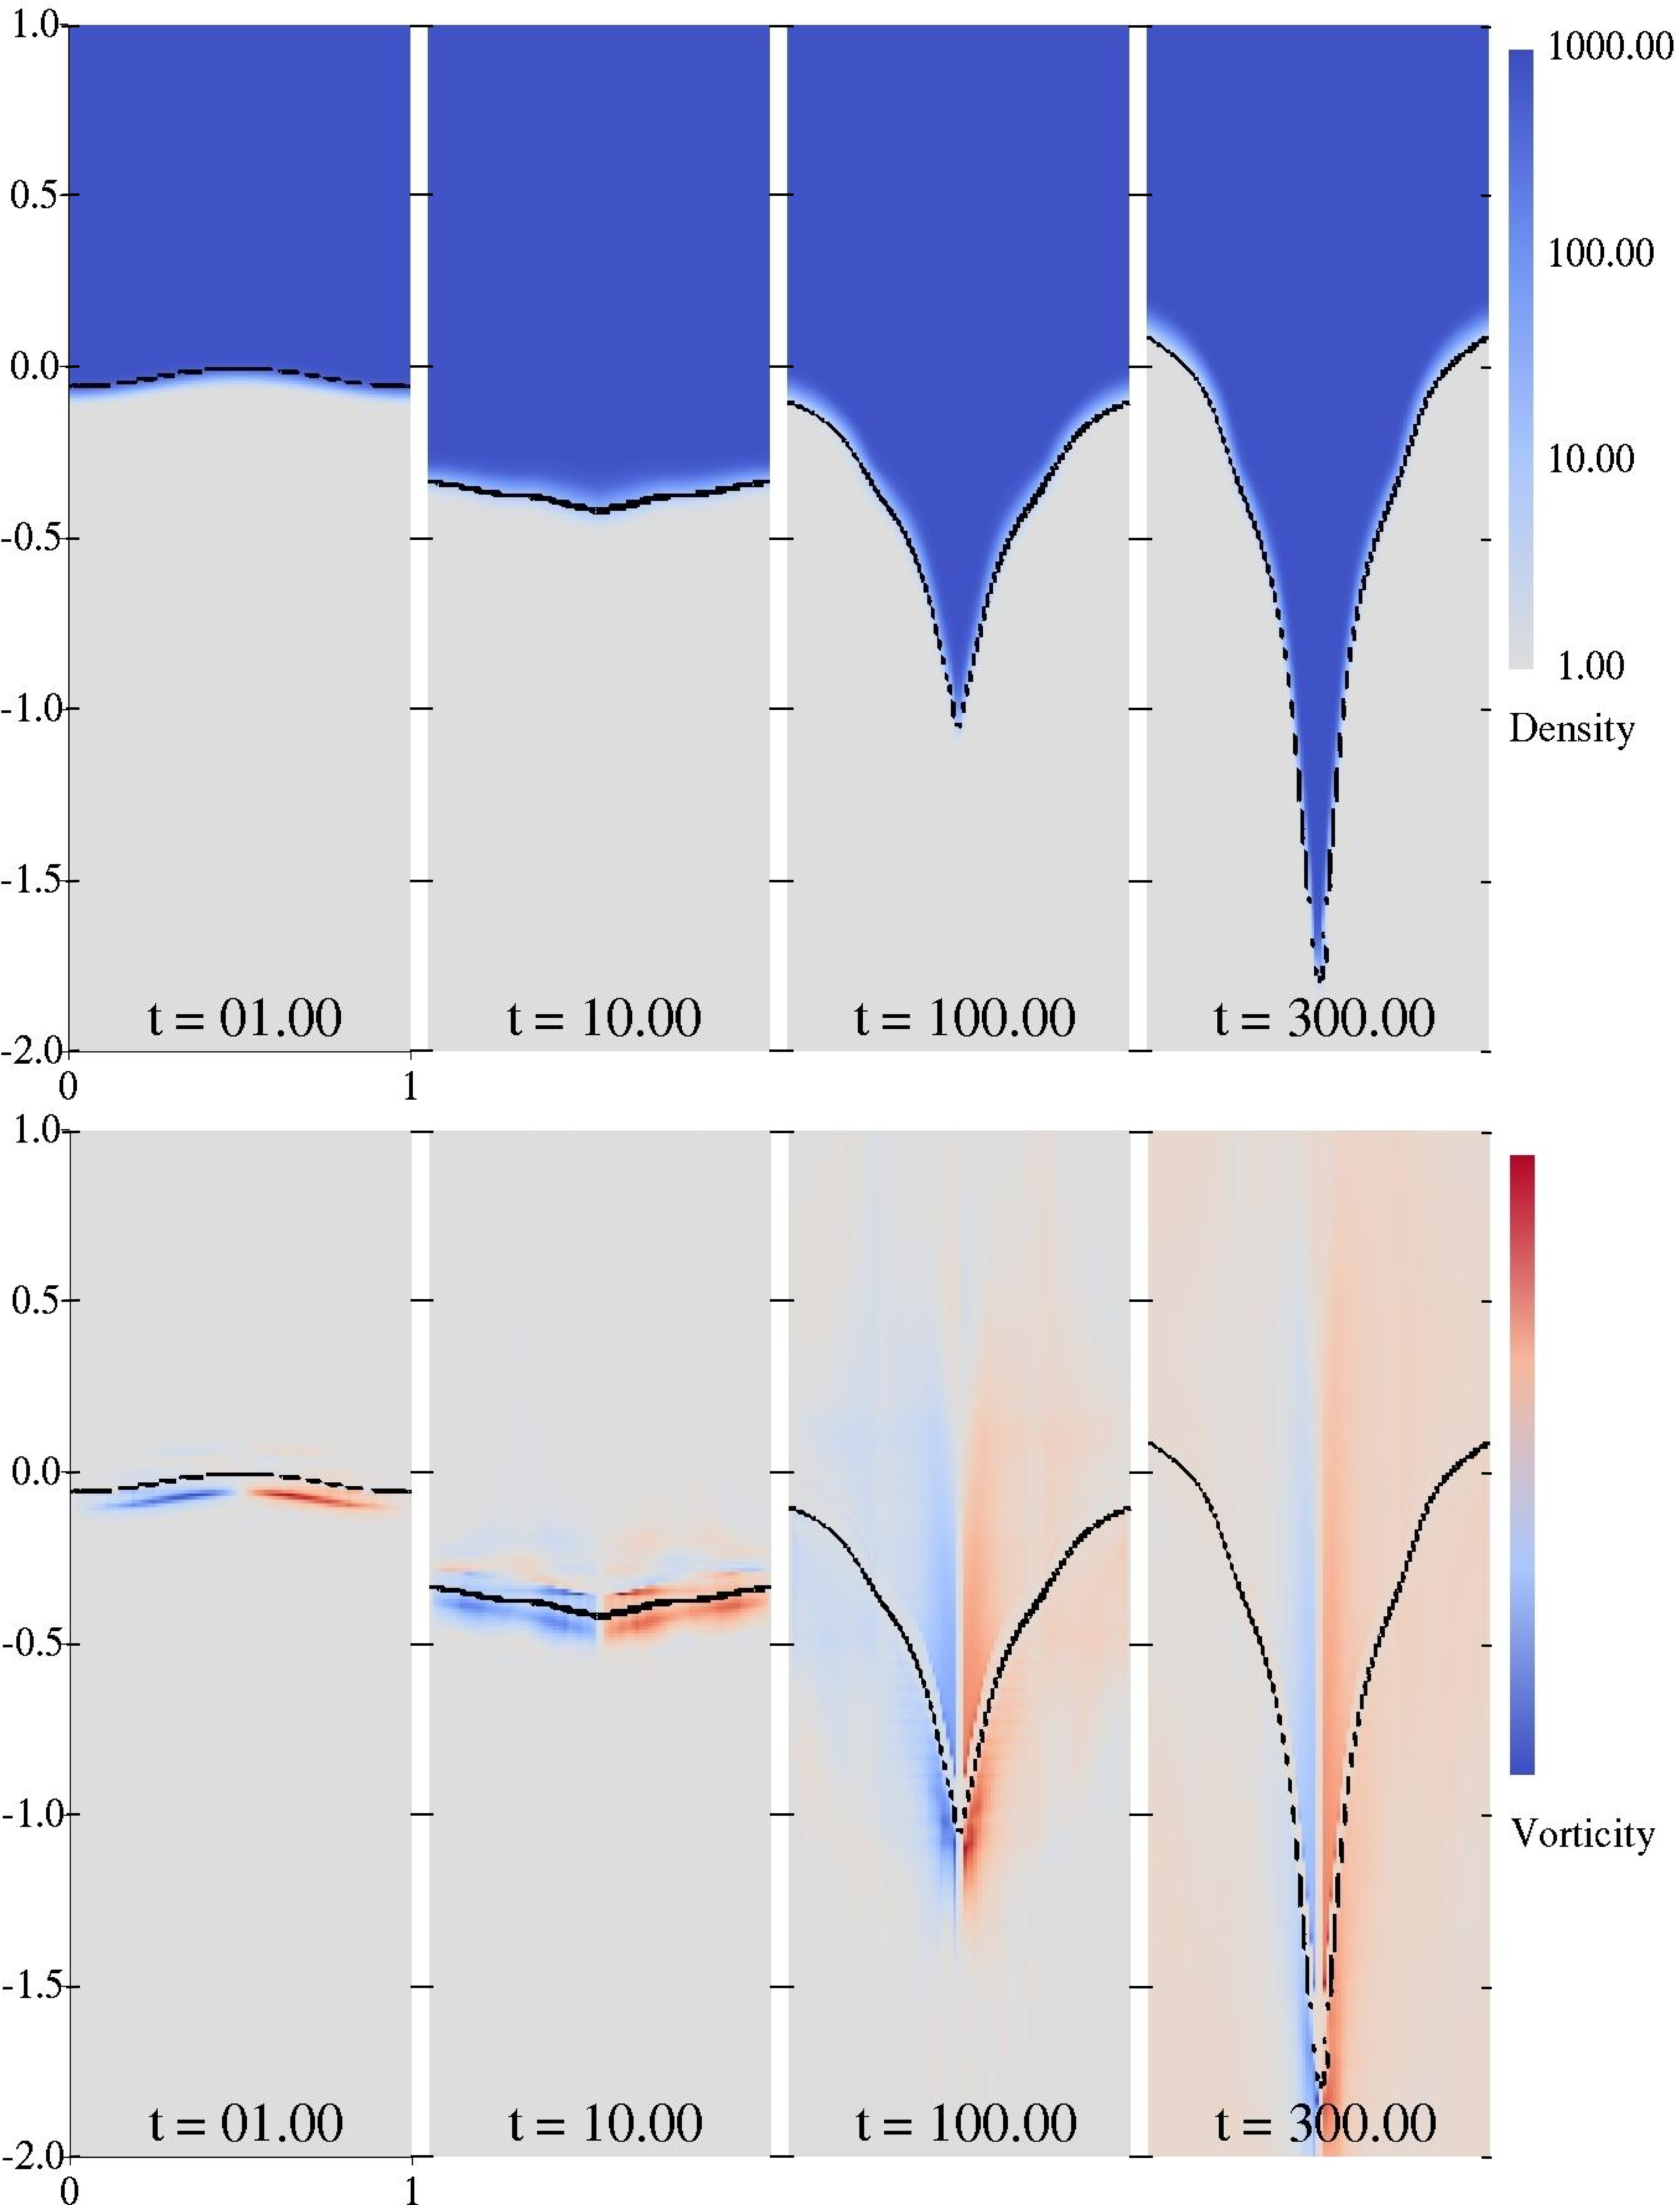
\includegraphics[width=0.9\textwidth]{./figs/lung_figs/snapshots_t1}
\caption[The evolution of the acoustically perturbed interface and vorticity field]{Surface plots of density (Top) and vorticity (Bottom)
  throughout the evolution of the interface for the $10$ MPa
  trapezoidal wave case. Areas of high density (i.e., water) are
indicated in dark blue. Areas of low density (i.e., air) are indicated
in white.  Positive (counterclockwise) vorticity is indicated in red,
and negative (clockwise) vorticity can be seen in blue.}
  \label{fig:interface_snapshots}
\end{figure}
%
\begin{figure}[h] 
  \centering
  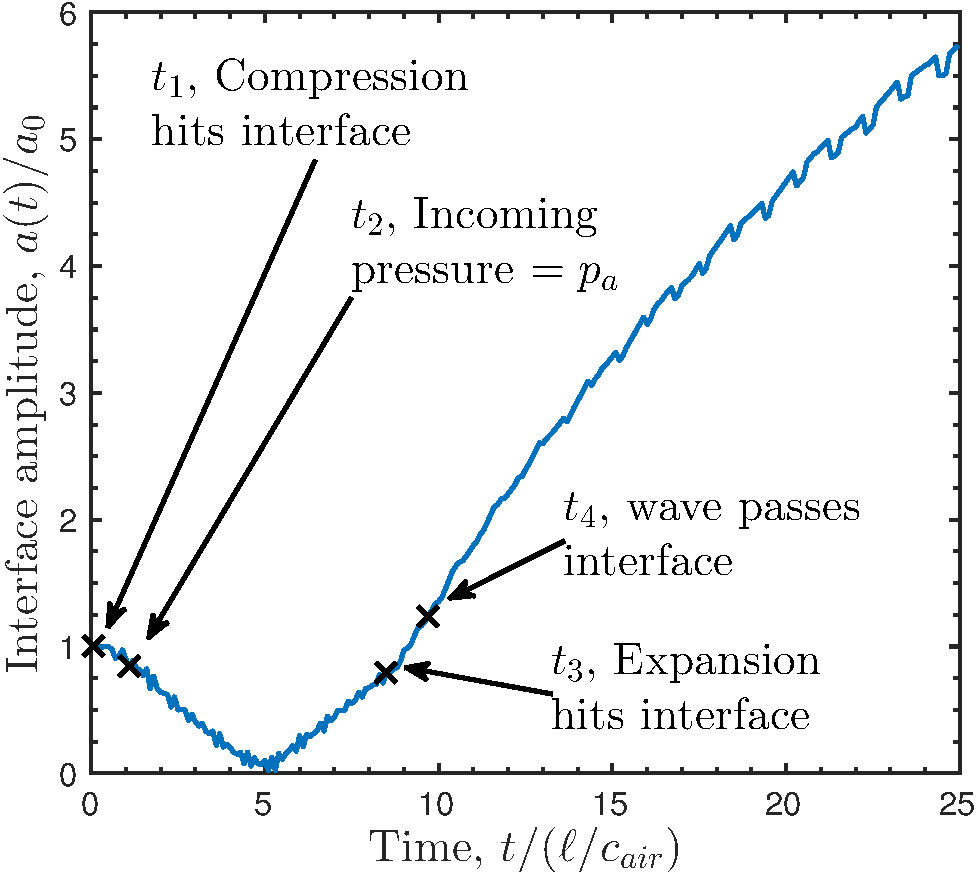
\includegraphics[width=0.48\textwidth]{./figs/lung_figs/trapz10_intf_schematic}
  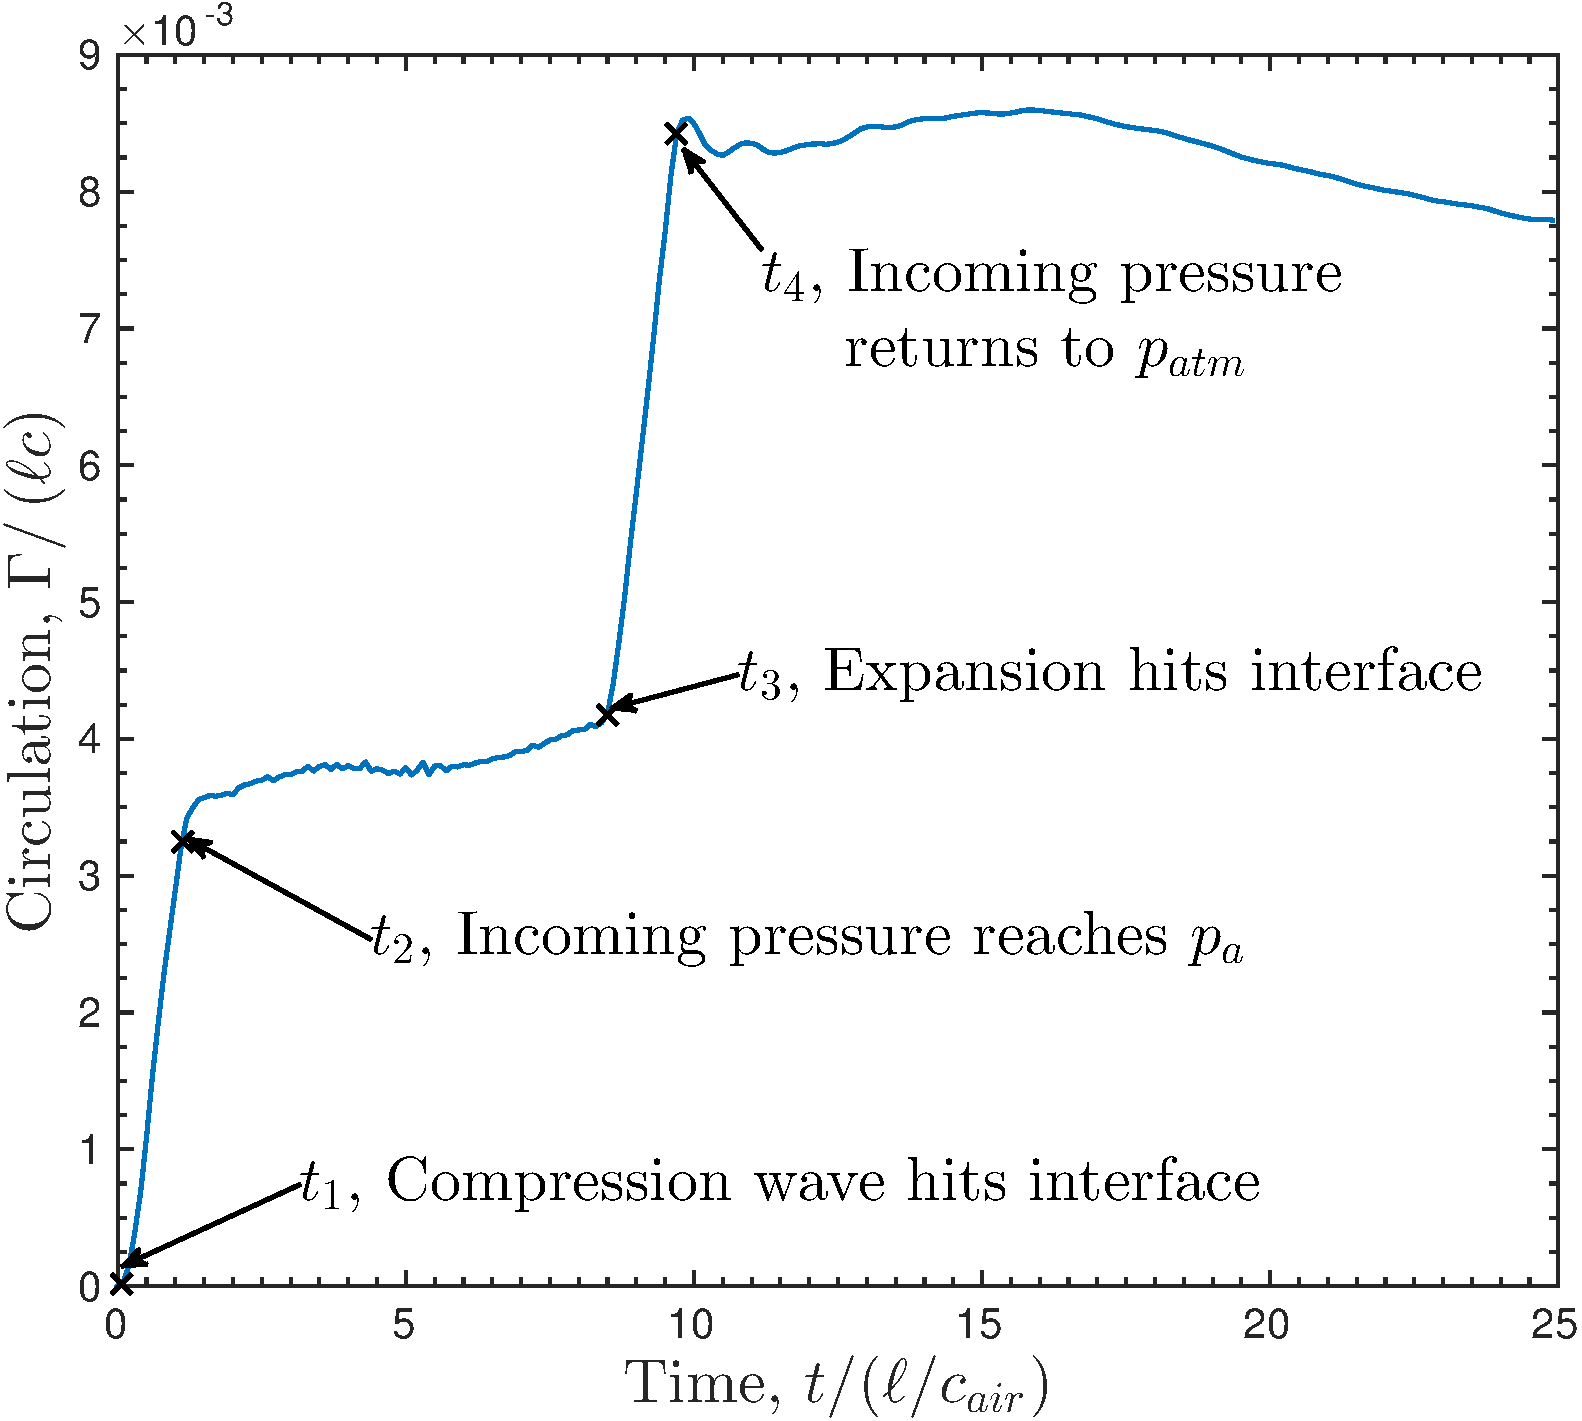
\includegraphics[width=0.48\textwidth]{./figs/lung_figs/trapz10_circ_schematic}
  \caption[The interface amplitude and circulation histories for the $10$ MPa trapezoidal wave]{The interface amplitude (left) and circulation (right)
    histories corresponding to the $10$ MPa trapezoidal waves are
    shown for $t\leq25$. Indicated times, $t_{1-4}$, are the times at
    which different stages of the incoming trapezoidal pressure wave
    shown in Figure \ref{fig:p0} first encounter the interface.}
  \label{fig:trapz10_circ_interface}
\end{figure}
%
%
\subsubsection{Dependence on acoustic wave amplitude}%
\label{subsubsec:amplitude_dependence}%
To investigate the dependence of the dynamics on the trapezoidal wave
amplitude, we compare results for $p_a=1$, $5$, and $10$ MPa while
keeping the initial lengths of the wave $L$ and the rise and fall
$\Delta L_a$ constant such that $p_a$ scales linearly with the
acoustic pressure gradient. Figure
\ref{fig:trapz_circ_interface_early}, illustrates the interface
amplitude and $p_a$-normalized circulation histories for $t\leq25$,
during and shortly after the wave-interface interaction. Black
$\bs{\times}$s along the curves indicate $t_{1-4}$, described
previously in Subsection \label{subsec:Qualitative}. During the
interaction between the interface and the compression wave, the rate
at which the perturbation amplitude decreases is greater for higher
amplitude waves. The circulation deposited during this period scales
linearly with $p_a$ as is consistent with baroclinically-generated
circulation based on our analysis. For the $10$ MPa wave, the phase of
the interface inverts at, before the expansion hits, causing
circulation deposited by the expansion to have the same sign as that
deposited by the compression. For the $1$ and $5$ MPa waves interface
phase inversion occurs after the expansion and consequently deposits
circulation opposite that of the compression wave.

Figure \ref{fig:trapz_circ_interface_loglog} \hl{(update this figure)}
shows the interface amplitude and circulation histories for $5$ and
$10$ MPa trapezoidal wave cases for $0 \leq t\leq 1000$. The
perturbation amplitude history is plotted on logarithmically-scaled
axes. For both waves, the slope of the perturbation amplitude is
approximately $0.60$ long after the waves have left the
interface. This is slightly higher than the 0.5 slope predicted by
scaling law \eqref{eq:intf_circ_scaling}. The results for the $1$ MPa
trapezoidal wave were not included because interface evolved too
slowly to obtain useful data given the computational resources available.
%
\begin{figure}[h] 
  \centering
  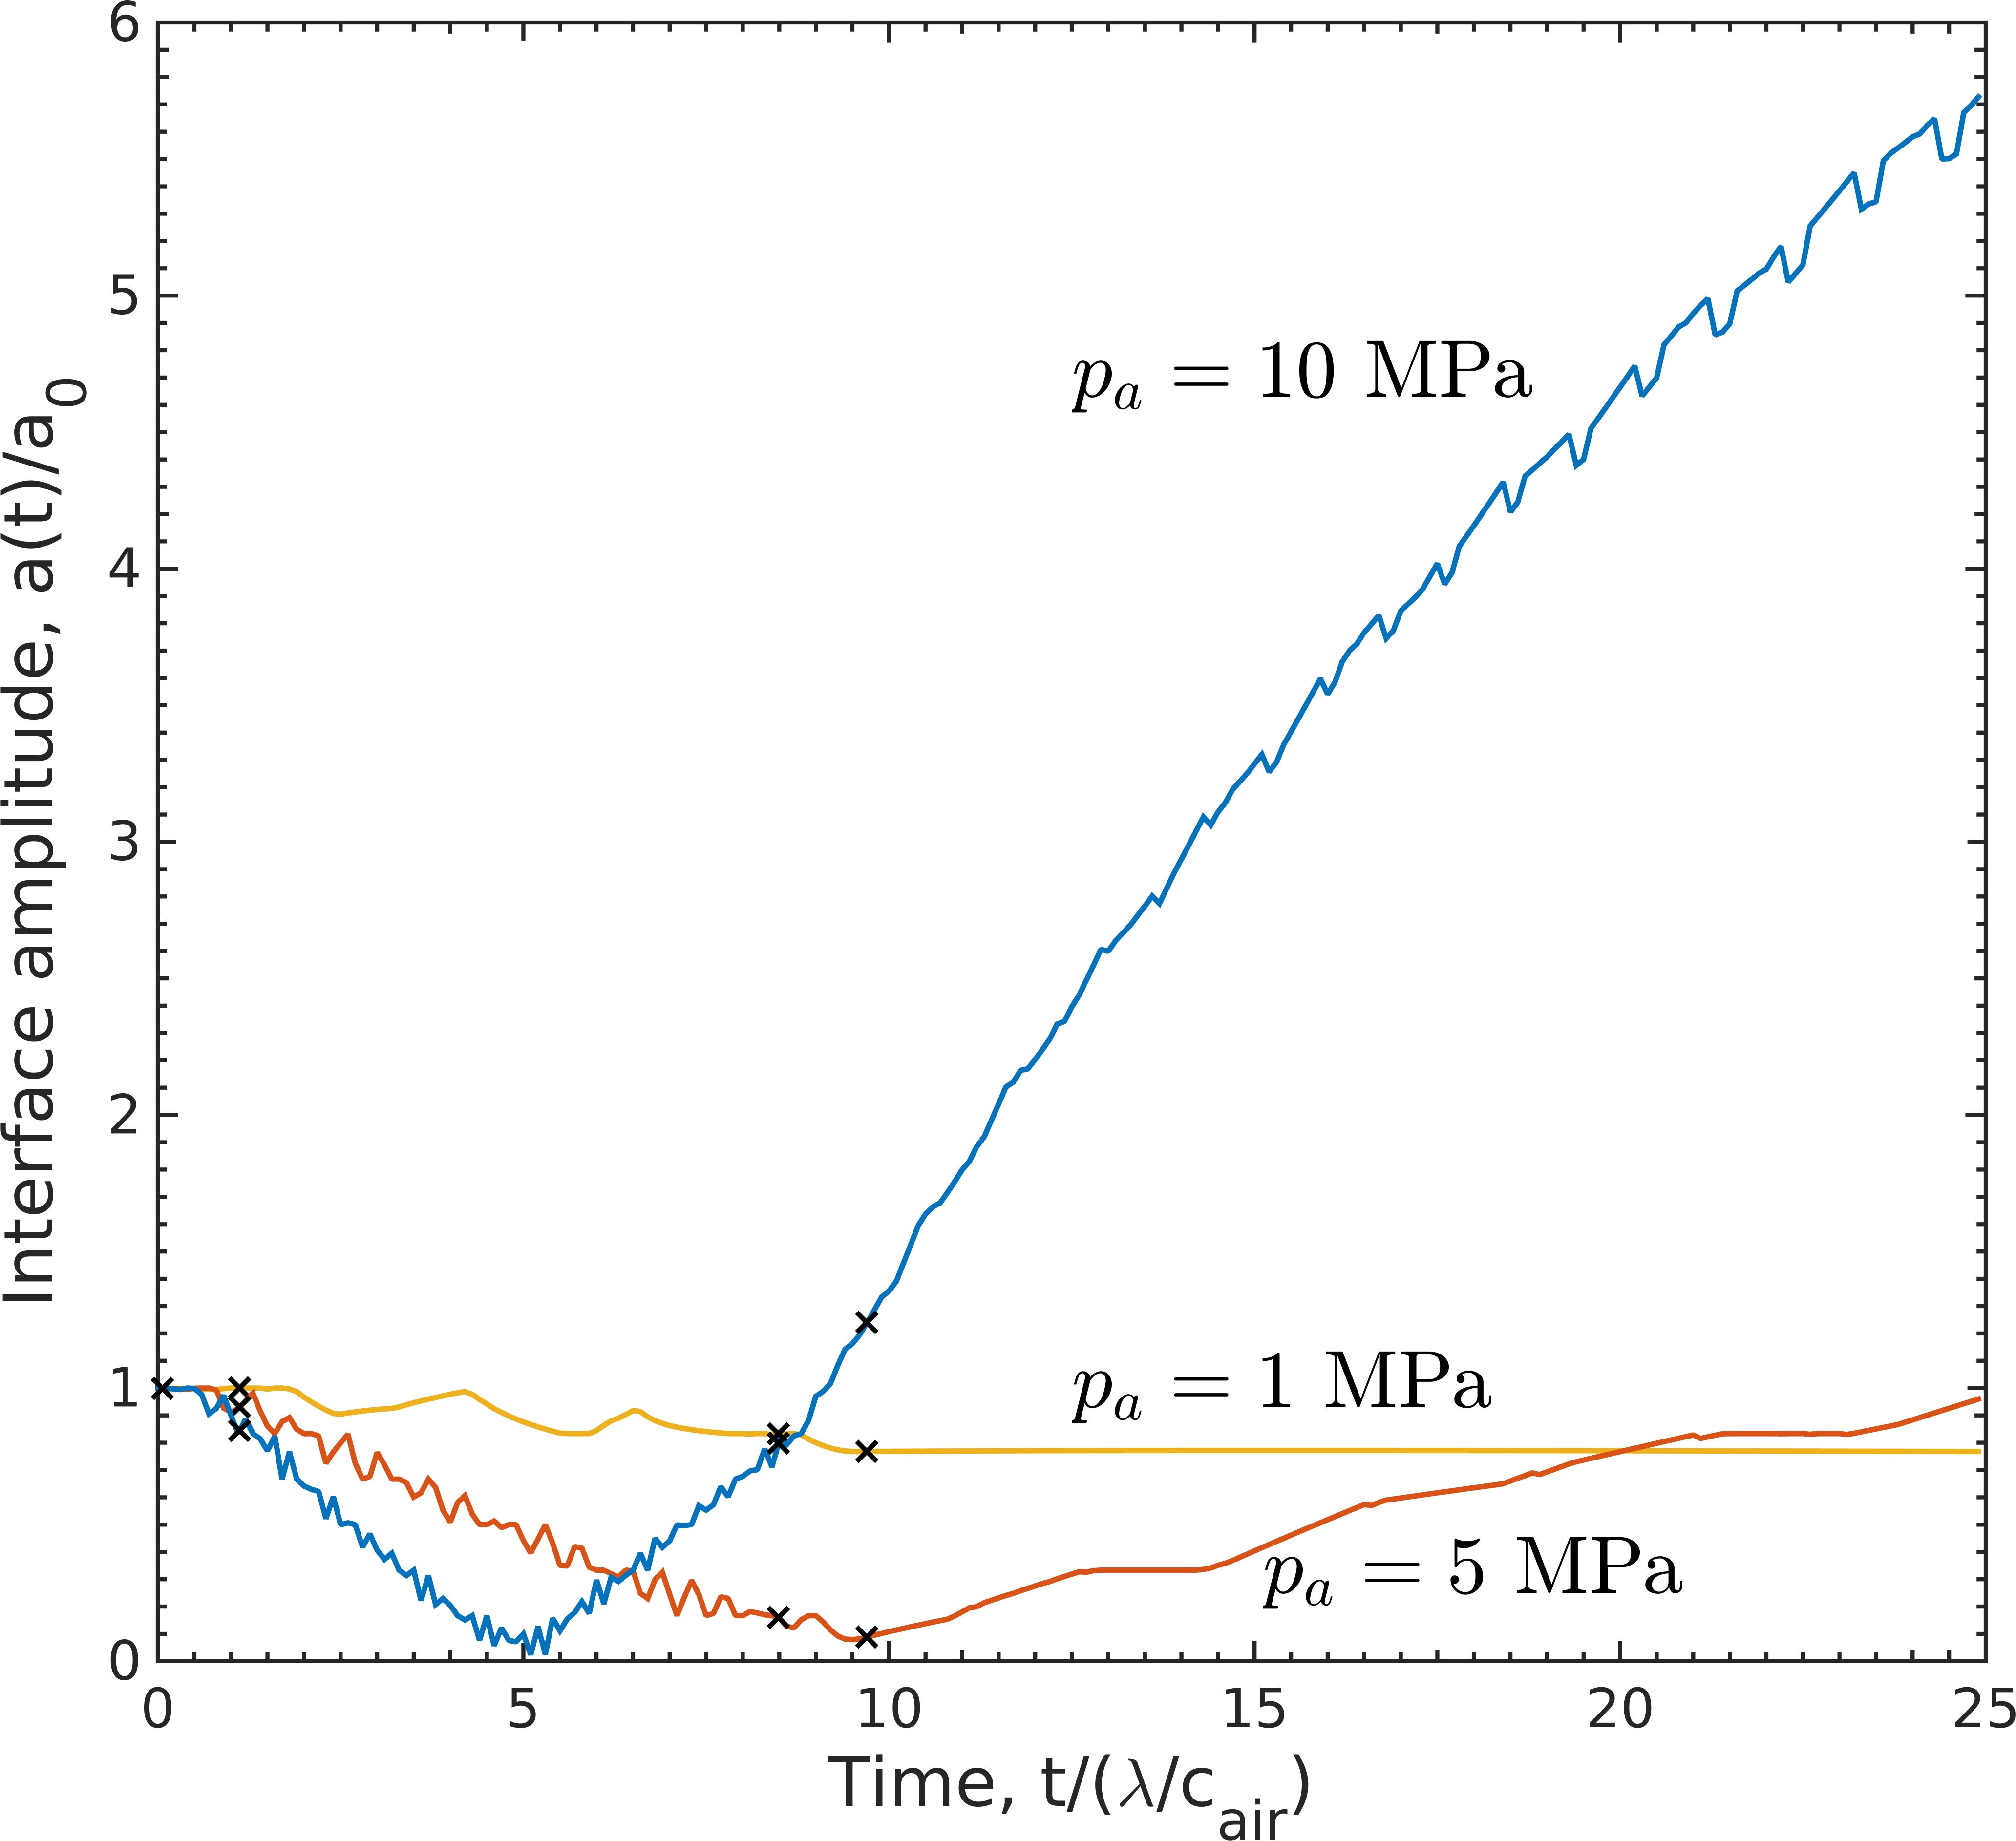
\includegraphics[width=0.48\textwidth]{./figs/lung_figs/interface_multi-amp_norm}
  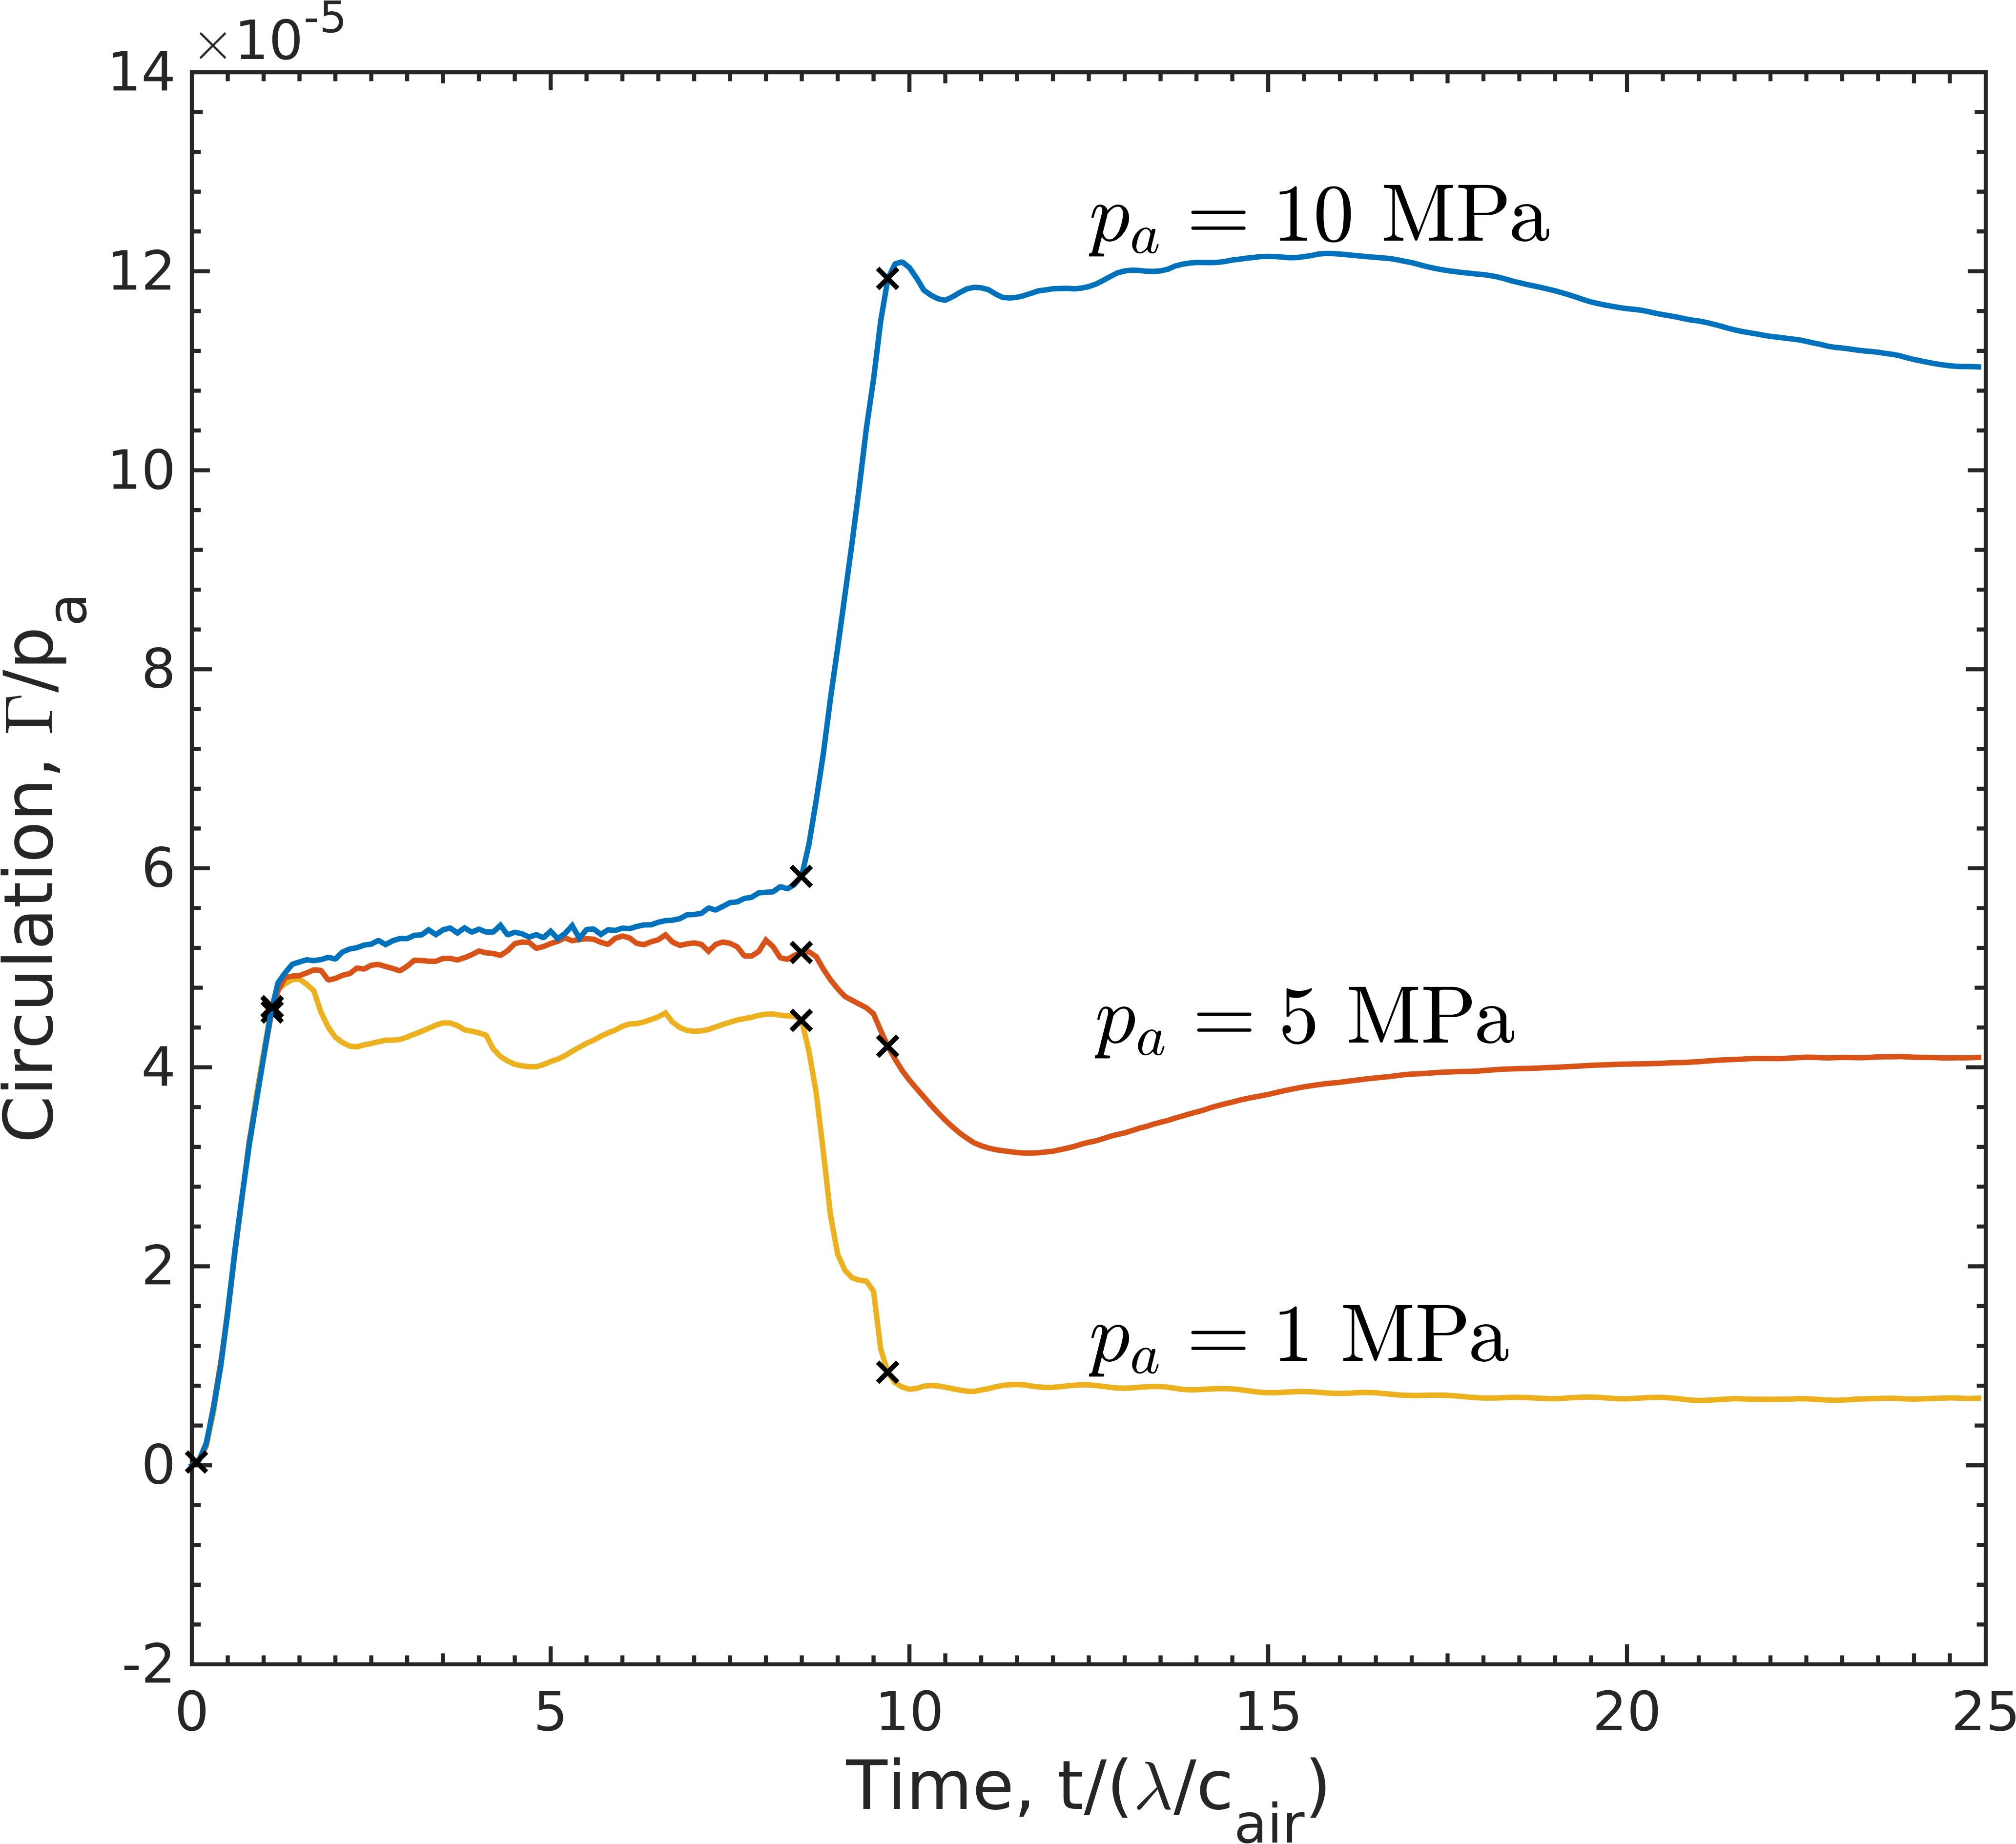
\includegraphics[width=0.48\textwidth]{./figs/lung_figs/circulation_multi-amp_norm}
  \caption[The interface and circulation dependence on wave amplitude at early time]{The interface amplitude (left) and circulation (right)
    histories corresponding to the $1$(yellow), $5$(orange), and
    $10$(blue) MPa trapezoidal waves are shown for $t\leq 25$. The
    circulation history is normalized by the acoustic amplitude of the
    incoming wave to illustrate that circulation deposition by the
    compression wave scales linearly with $p_a$.}
  \label{fig:trapz_circ_interface_early}
\end{figure}
%
\begin{figure}[h] 
  \centering
  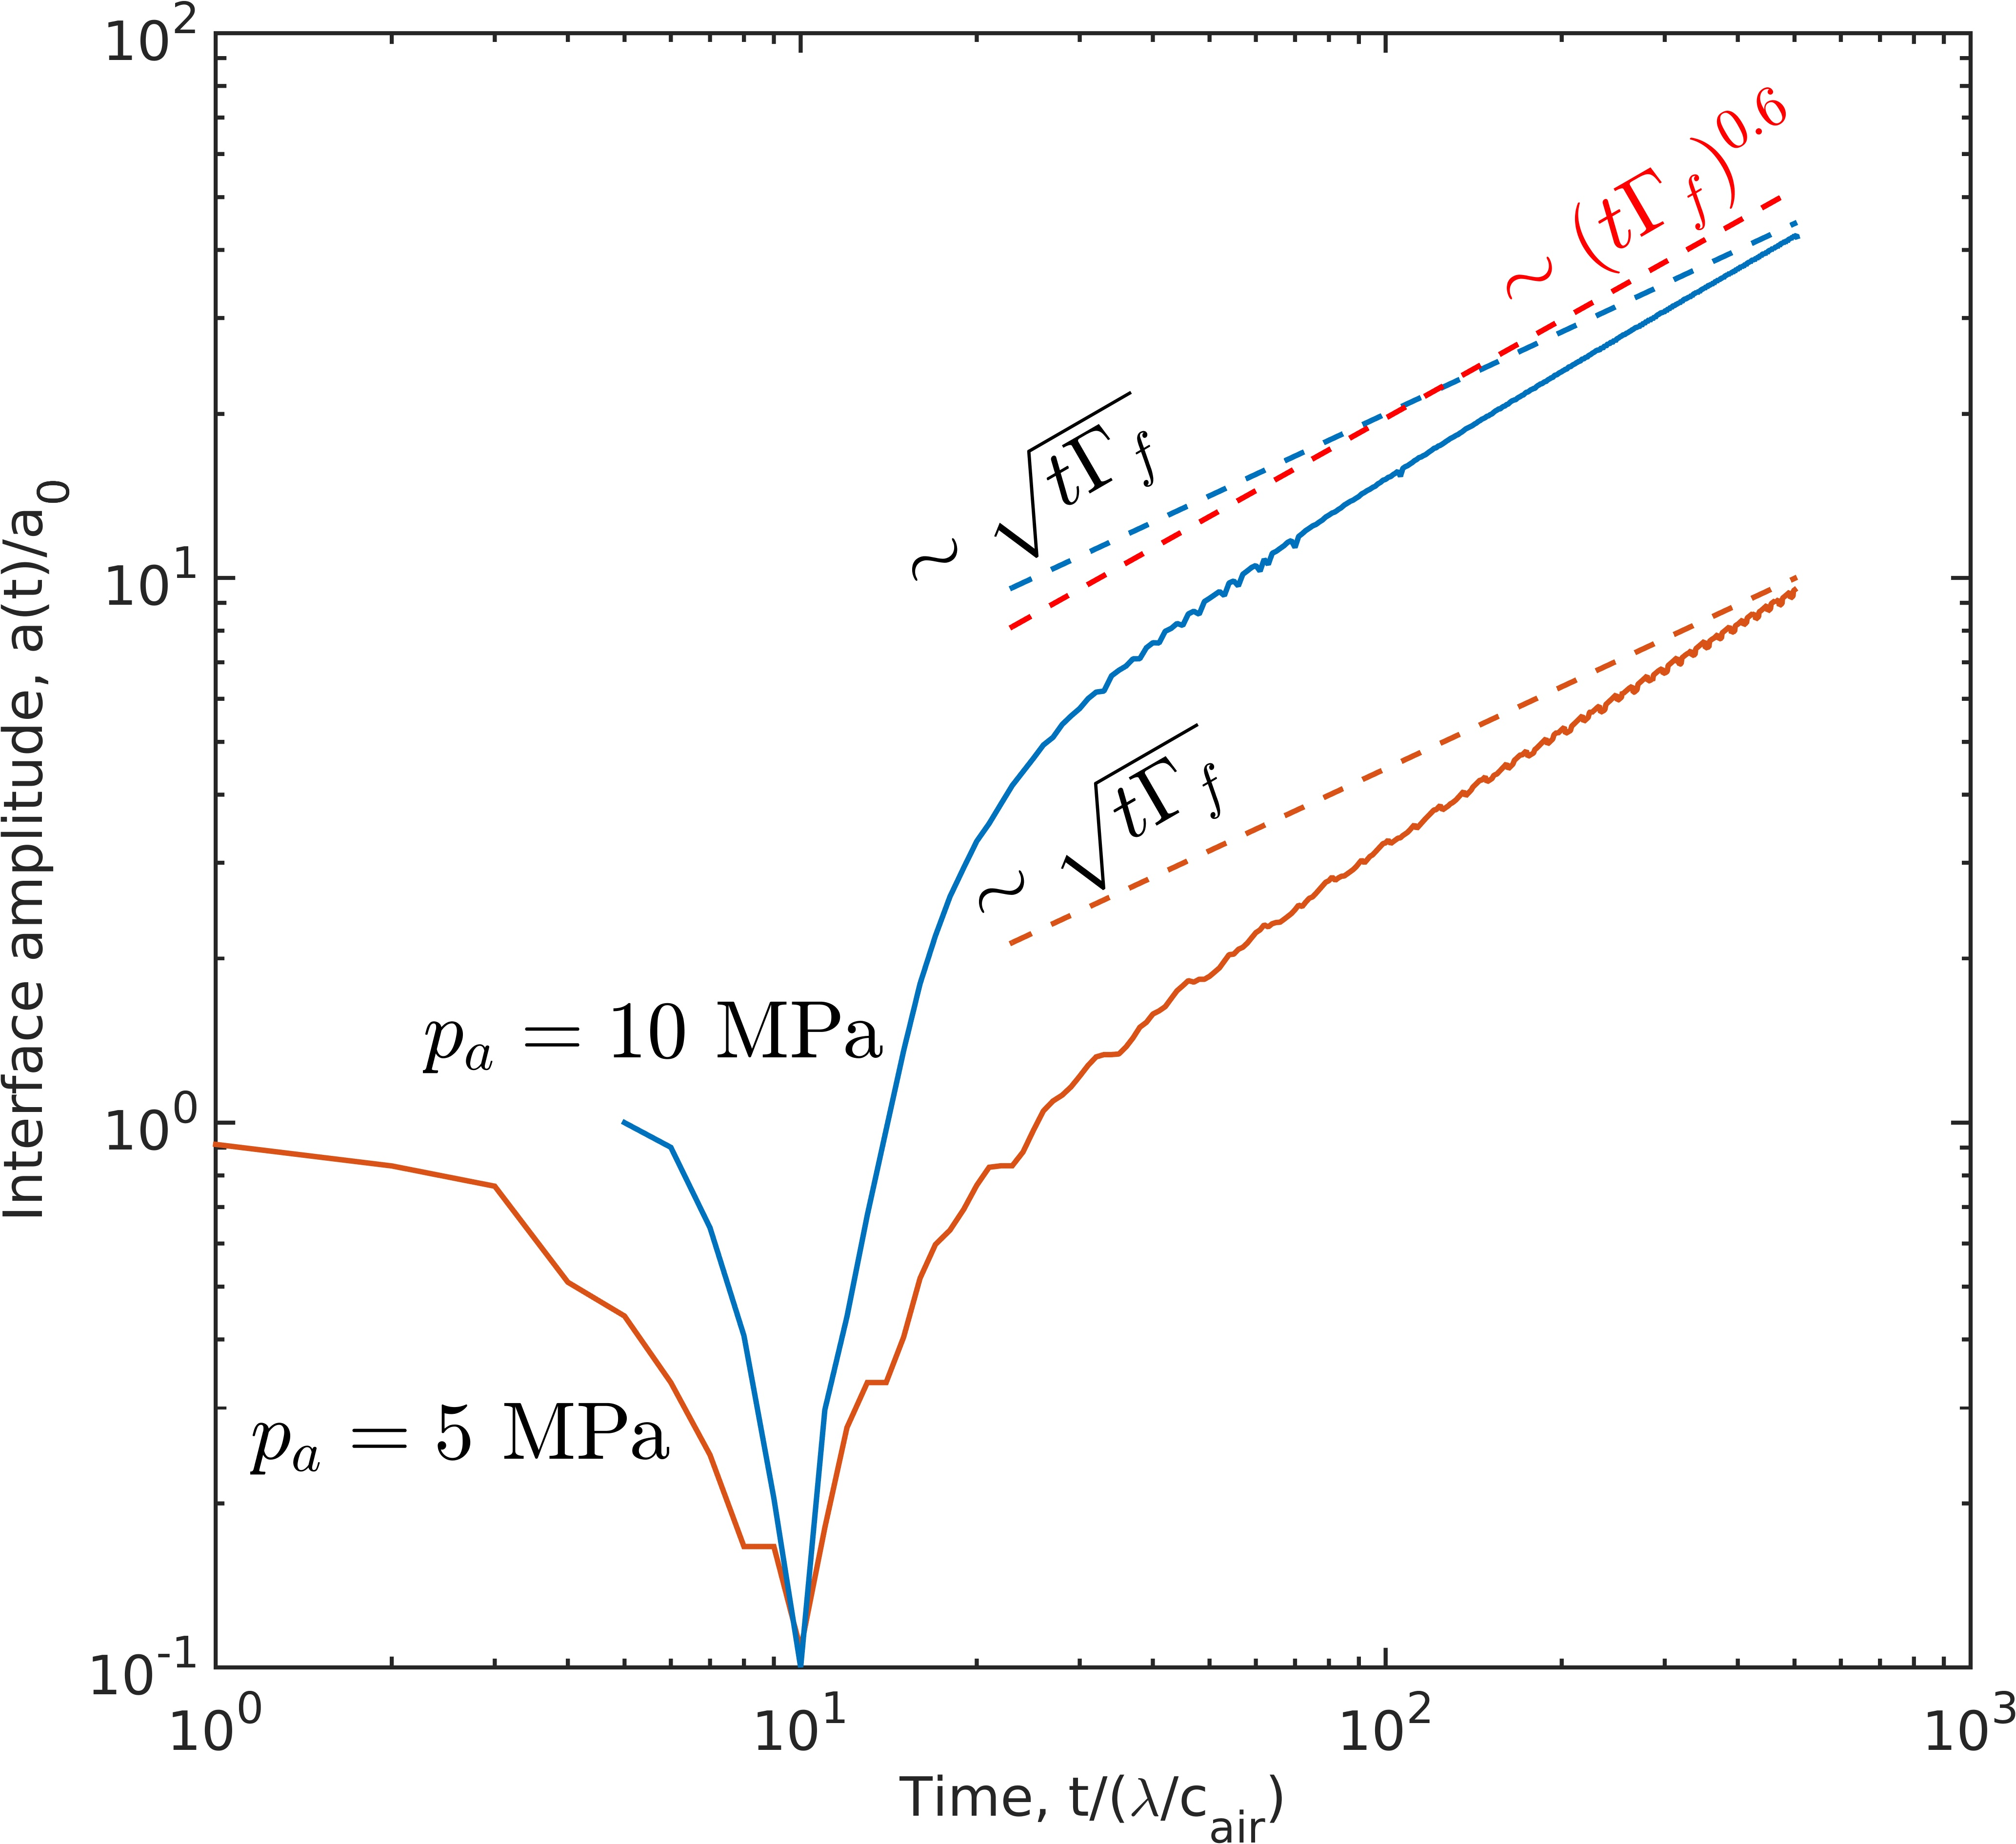
\includegraphics[width=0.48\textwidth]{./figs/lung_figs/interface_multi-amp_loglog_roe_extra}
  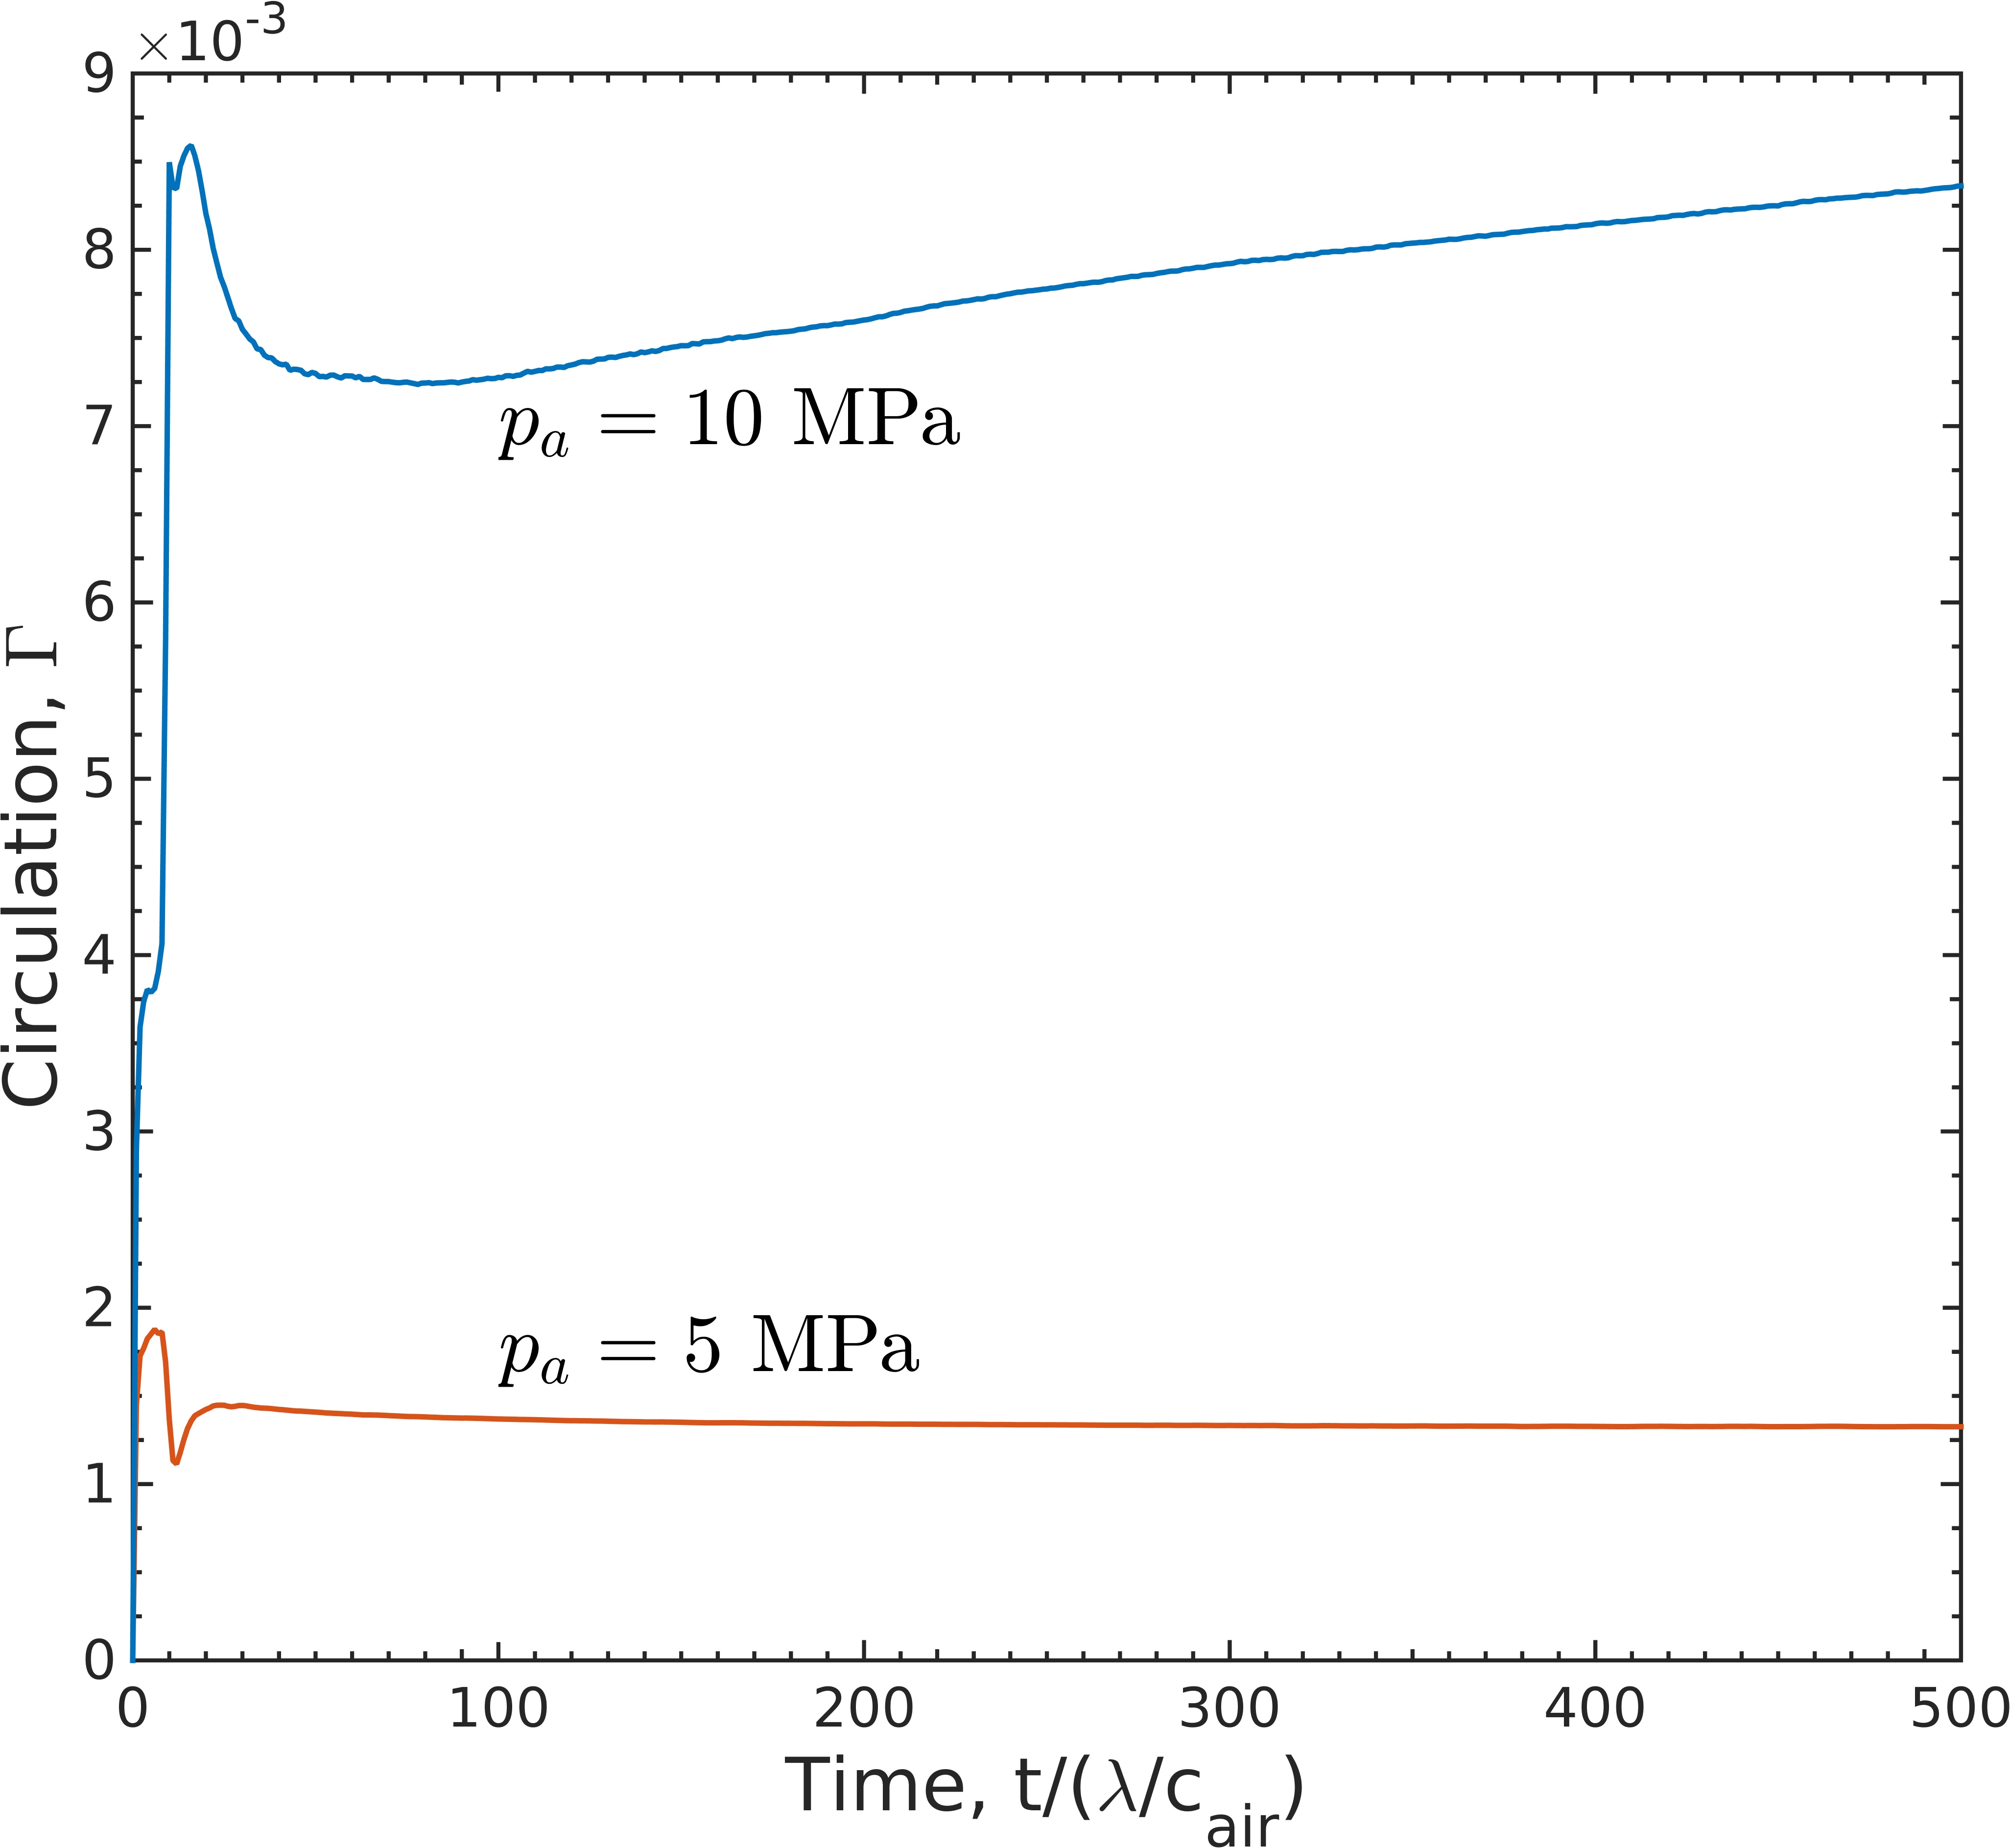
\includegraphics[width=0.48\textwidth]{./figs/lung_figs/circulation_multi-amp2_roe}
  \caption[The interface and circulation dependence on wave amplitude
  at long time]{The interface amplitude (left) and circulation (right)
    histories corresponding to the $5$(orange) and $10$(blue) MPa
    trapezoidal waves are shown for $t\leq 500$. To appropriately
    compare late time dynamics, time has been offset in the interface
    amplitude history such that the phase reversal appears to occur
    simultaneously in both simulations. Dashed lines of the same color
    are used to demonstrate the expected slope of pure circulation
    driven interface growth, based on Equation
    \eqref{eq:intf_circ_scaling}. The red dashed line shows the slope we
    appear to be approaching for the $10$ MPa wave case for the end time.}
  \label{fig:trapz_circ_interface_loglog}
\end{figure}
%
\subsubsection{Dependence on the length of the wave}%
To investigate the dependence of the dynamics on the length of the
trapezoidal wave $L$, and comparably the wave-interface interaction
time, we compare results for $p_a=10$ MPa waves of constant rise and
fall length $\Delta L_a$. This effectively changes the time the
interface has to evolve while experiencing the constant elevated
pressure portion of the wave between the compression and expansion.
Figure \ref{fig:trapz_circ_interface_multi-lag} shows the interface
amplitude and circulation histories corresponding to waves with
$L=45\lambda, 35\lambda ,30\lambda ,25\lambda ,15\lambda ,10\lambda$
for $0 \leq t\leq 25$.  For the three longest waves, $L \geq 30\lambda$,
the expansion encounters the interface after the perturbation reverses
phase. In these cases, the expansion deposits additional positive
circulation along the right half of the interface. For the shorter
waves, $L \leq 25\lambda$, the expansion encounters the interface before
the perturbation reverses phase and the net half-domain circulation is
decreased. Comparing cases in which the interface inverts phase before
the expansion occurs the larger $a(t)$ is at the time, the more
circulation is generated. The same is true when comparing cases in
which the phase inversion occurs after the interface inverts phase.
%
\begin{figure}[h] 
  \centering
  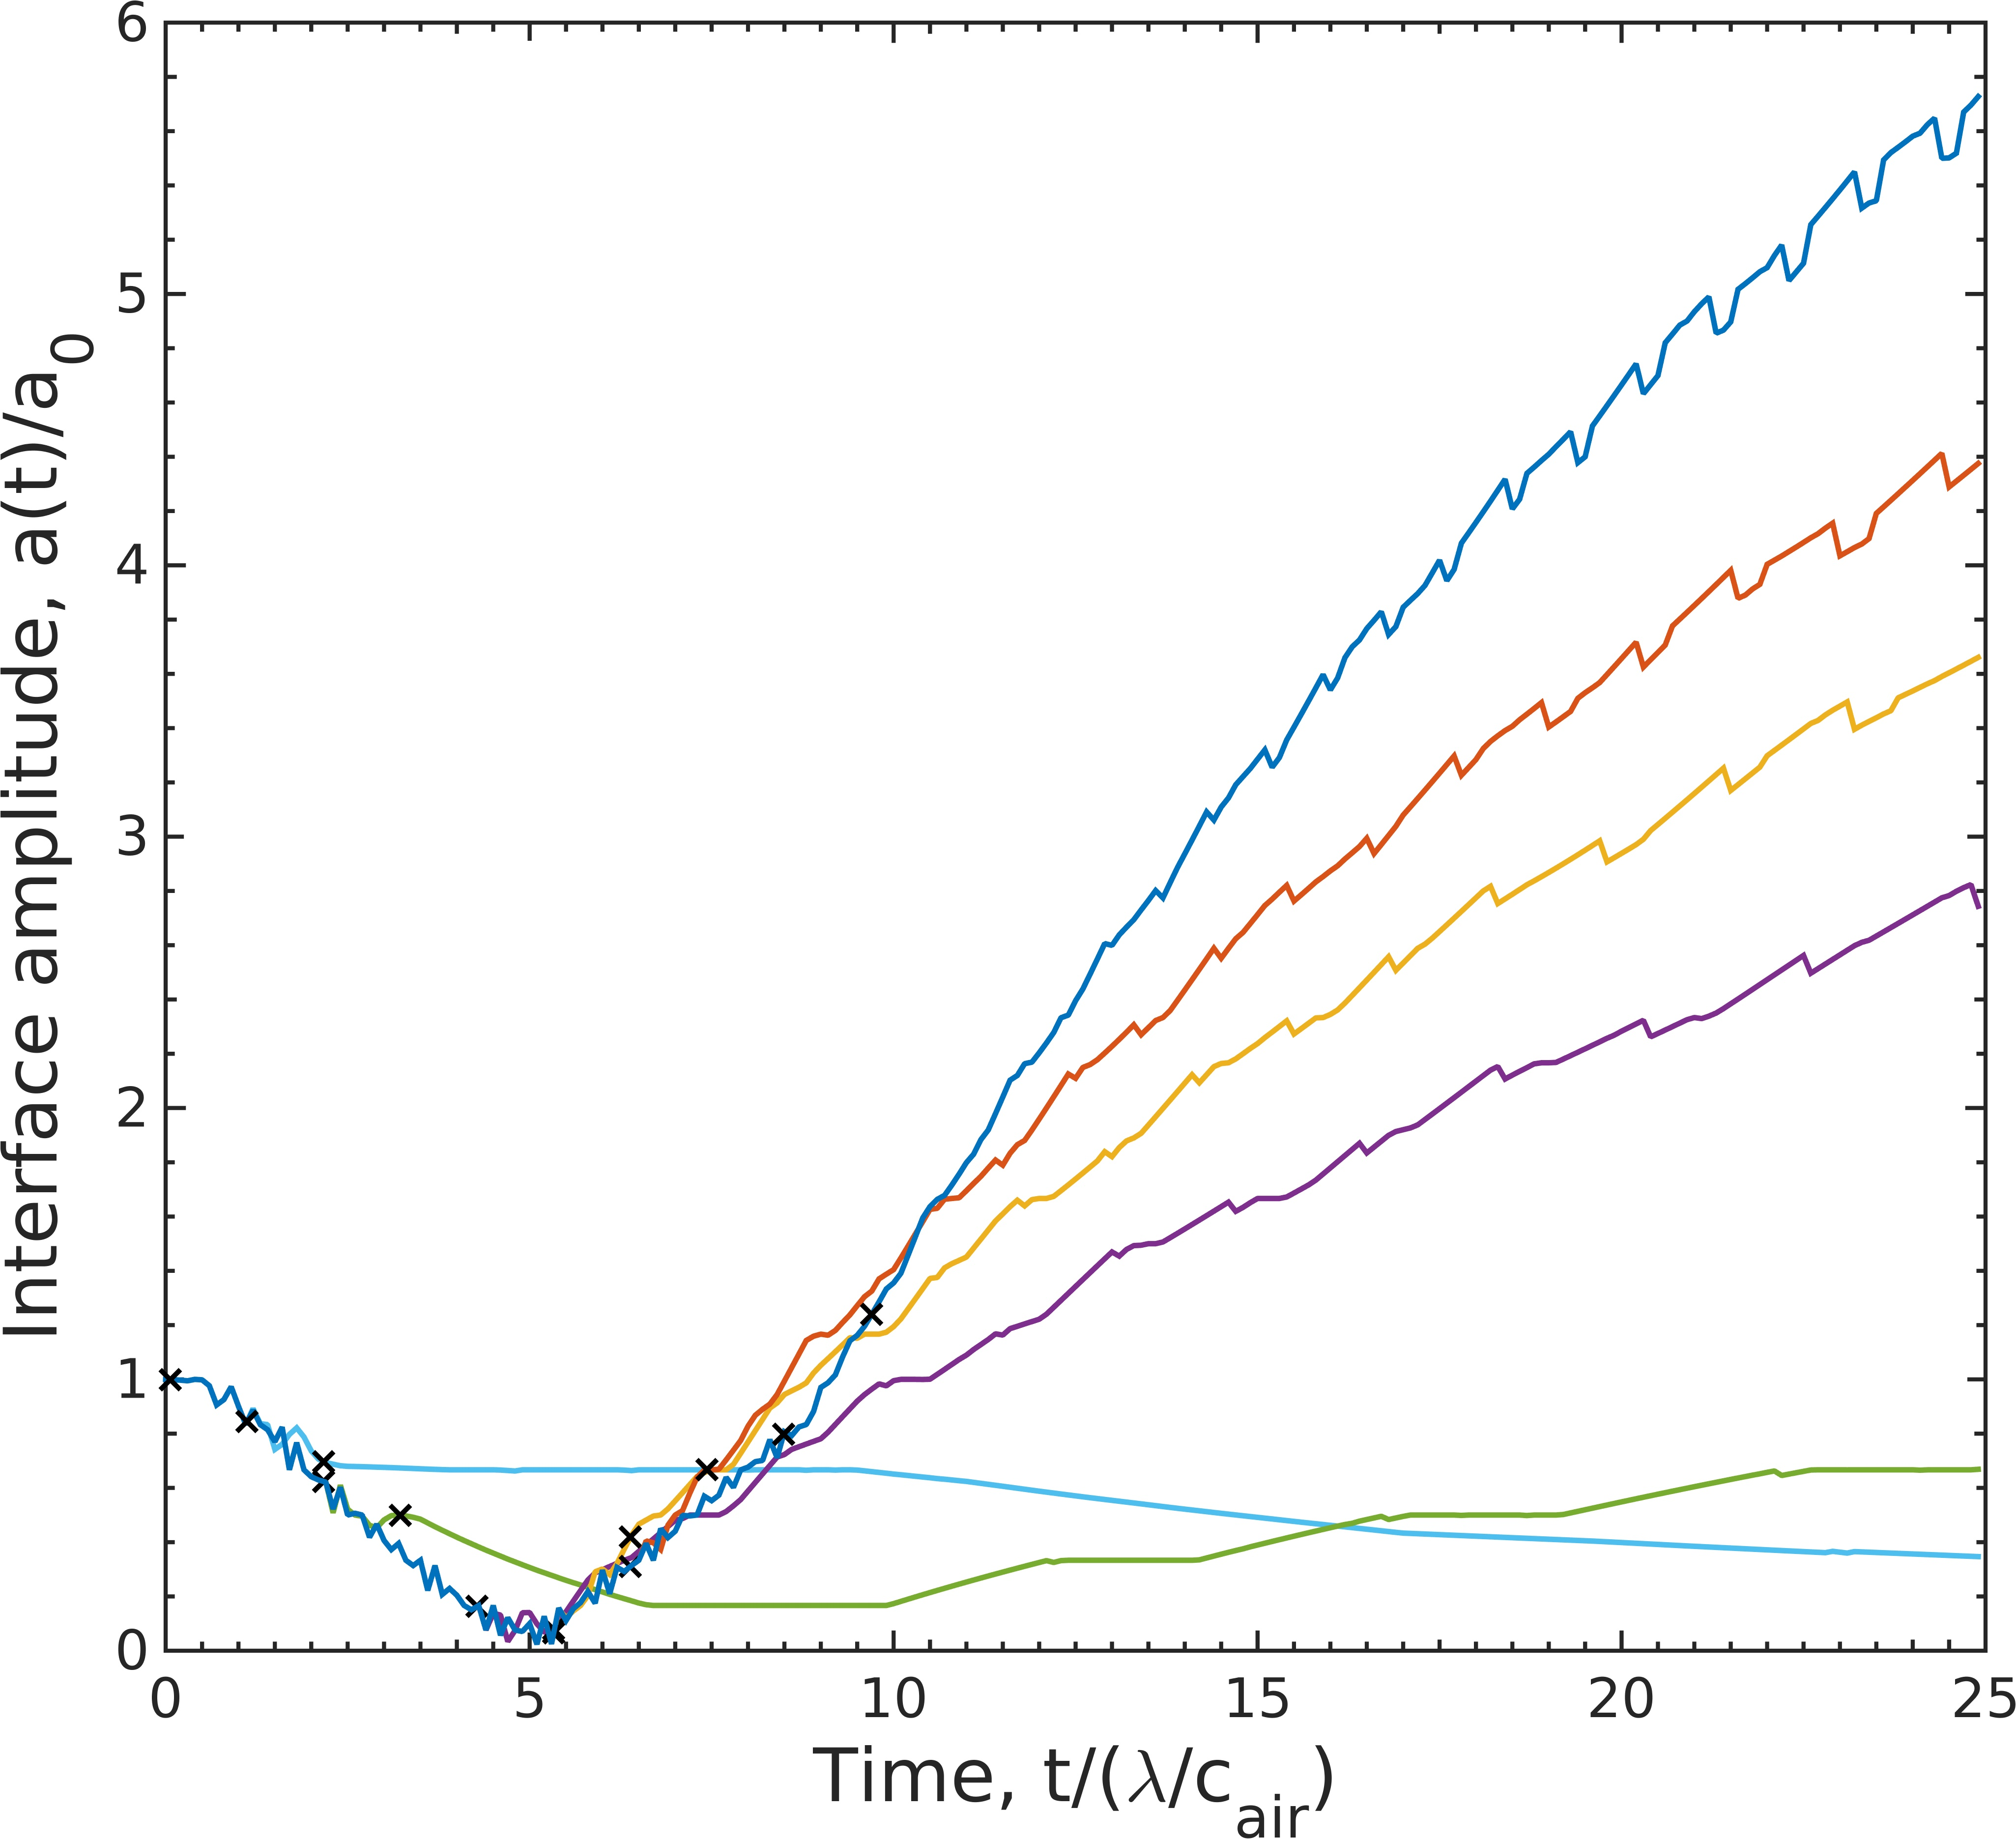
\includegraphics[width=0.48\textwidth]{./figs/lung_figs/interface_multi-lag}
  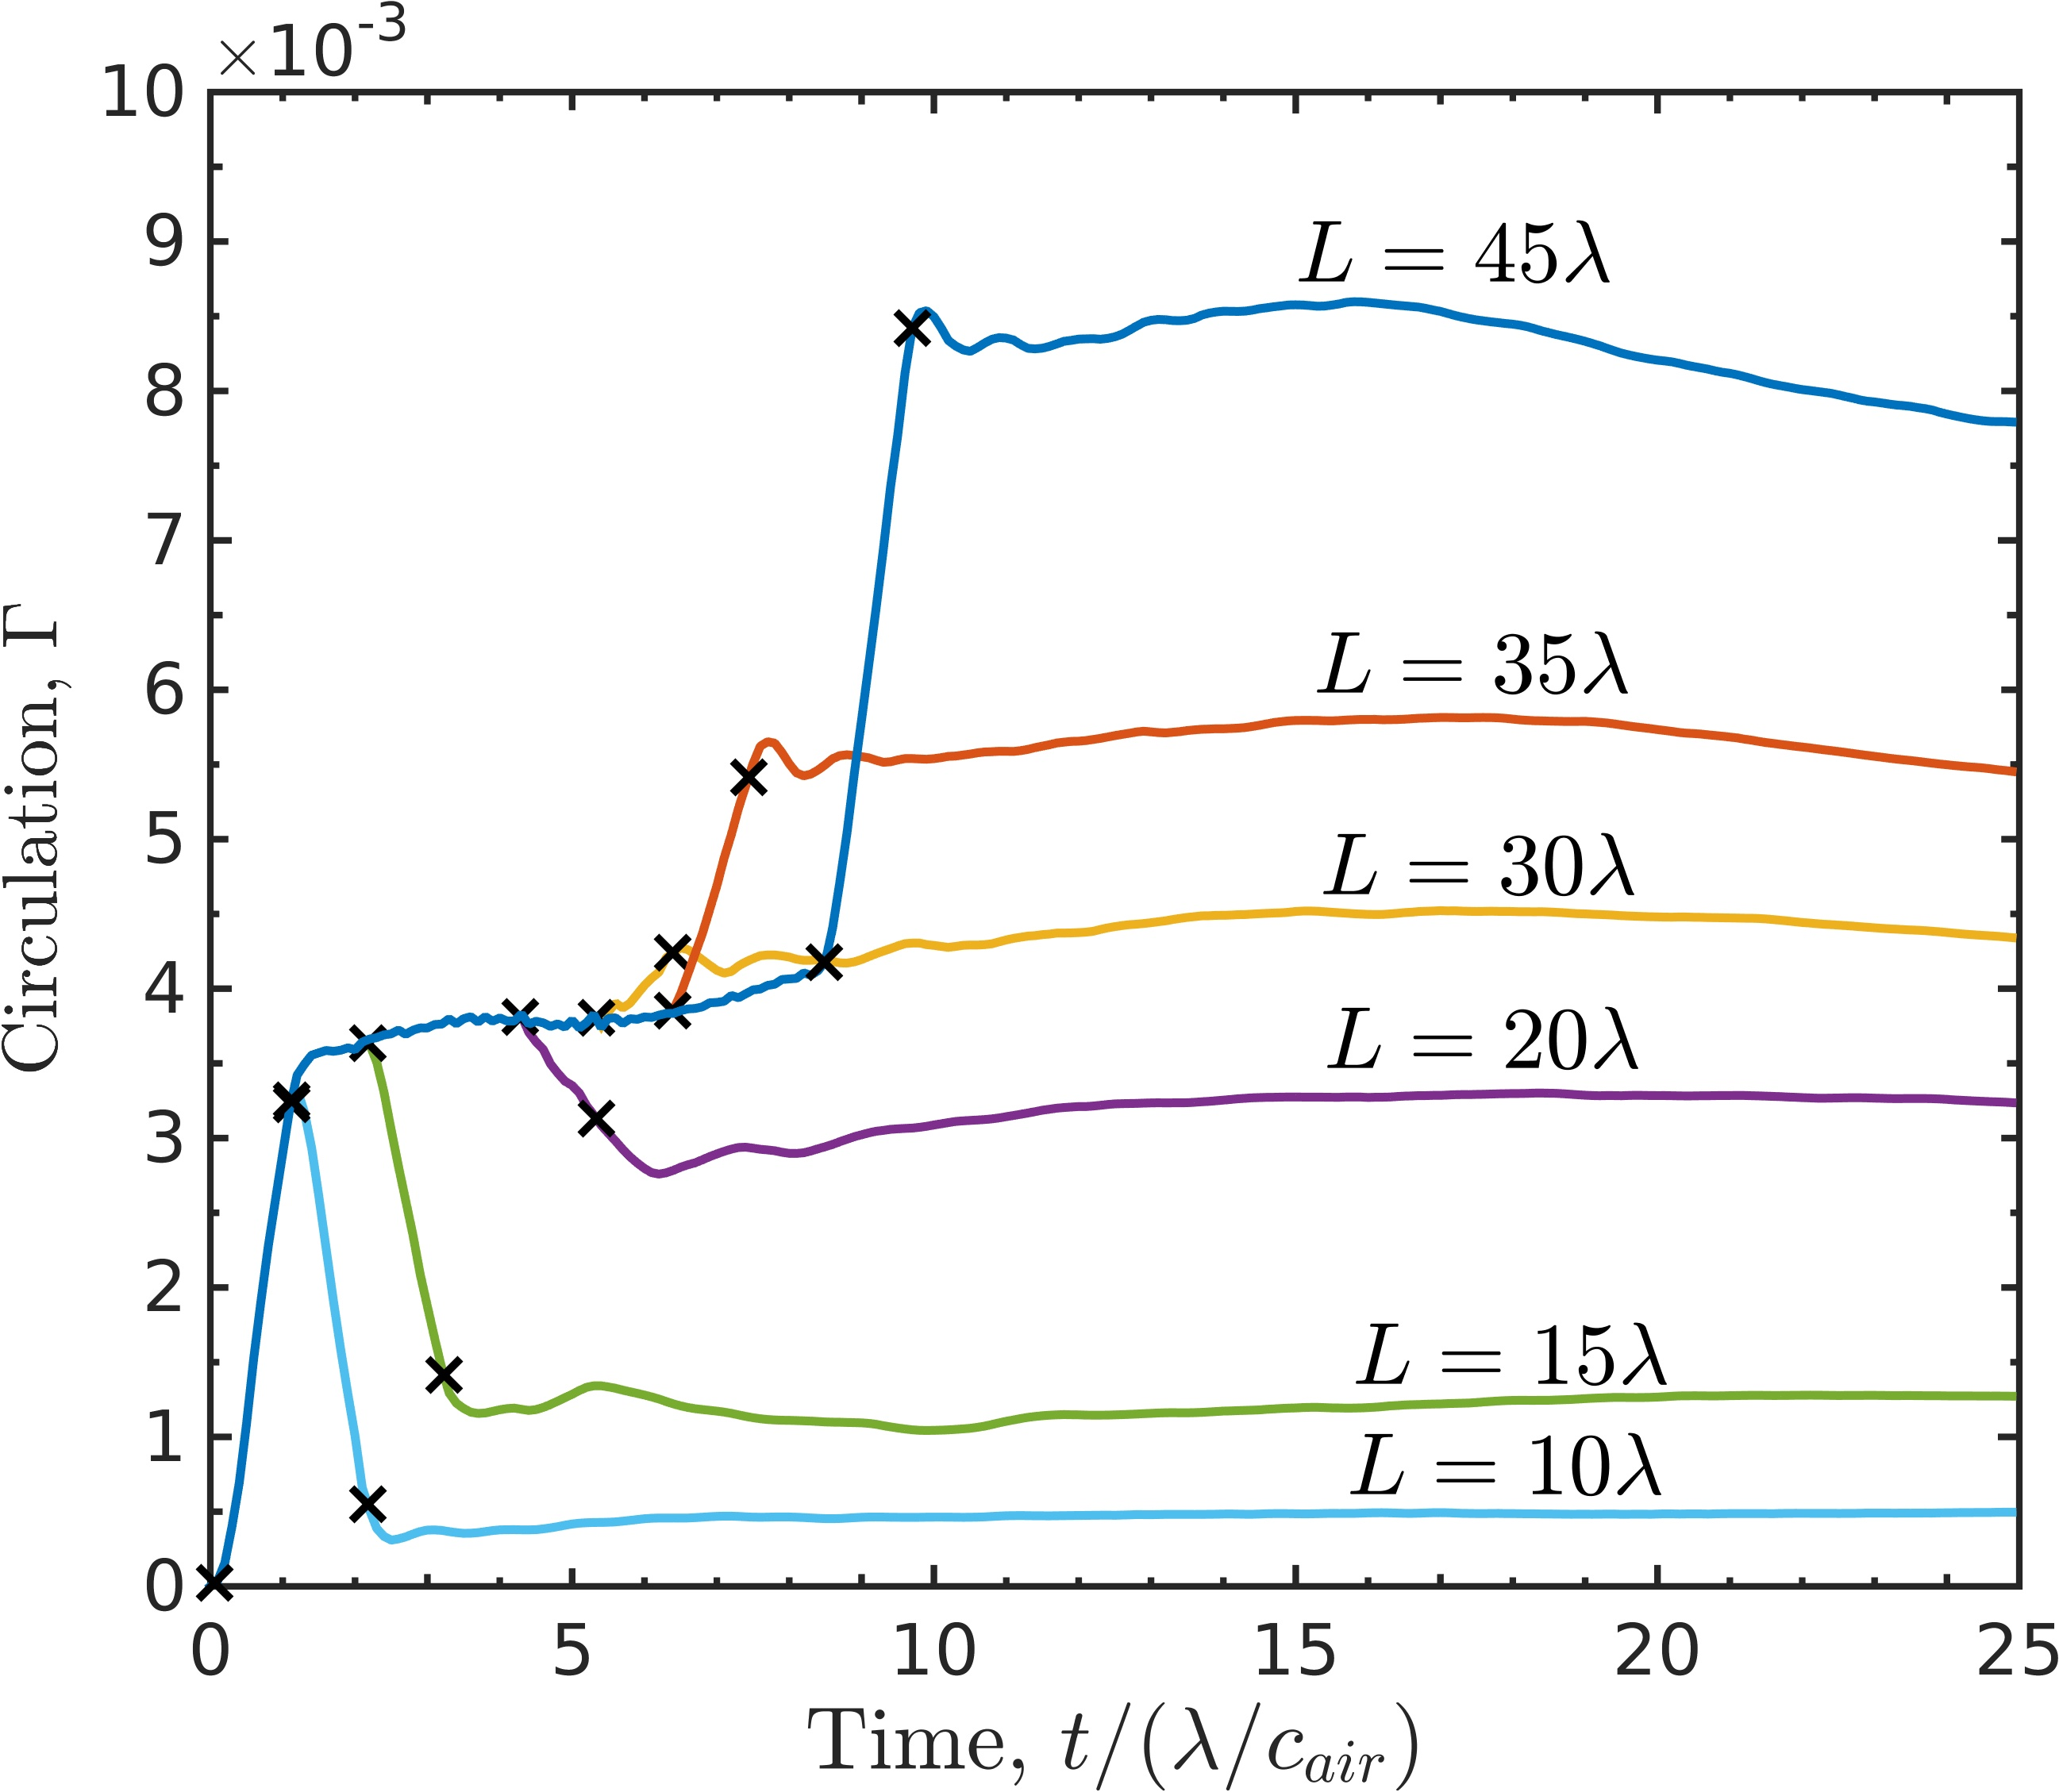
\includegraphics[width=0.48\textwidth]{./figs/lung_figs/circulation_multi-lag_fixed}
  \caption[The interface and circulation dependence on wave
  duration]{The interface amplitude (left) and circulation (right)
    histories for waves of varying total length $L$ and elevated
    static pressure duration between the expansion and compression
    . Here we show results for $L=45\lambda$ (blue), $L=35\lambda$
    (orange), $L=30\lambda$ (yellow), $L=20\lambda$ (purple),
    $L=15\lambda$ (green), $L=10\lambda$ (light blue)}
  \label{fig:trapz_circ_interface_multi-lag}
\end{figure}
%
\subsection{Discussion}
\label{subsec:discussion}
After the passage of the trapezoidal acoustic waves the pressure
returns to the initial, ambient conditions. This implies that the
integral of the pressure gradient $\nabla p$ along the interface, over
all time is zero. Hence we surmise that if the interface remains
unchanged during the interaction with the wave, as it would for a wave
moving with infinite velocity, $\nabla \rho$ would remain constant and
the net baroclinic circulation deposited must be zero. Thus for any
finite duration acoustic wave to deposit net baroclinic circulation
upon an interface, the interface itself must deform during interaction
with the wave. This deformation alters the misalignment of the
pressure and density gradients throughout the passage of the wave such
that vorticity deposited by the compression and expansion waves do not
cancel. Note that this of particular interest for waves in which
the pressure returns to the initial condition after the wave passes,
which is not the case for the traditional shock-accelerated \ac{RMI}
problem.

For the cases varying the length of the wave $L$, we previously noted
that whether the expansion increased or decreased the total
half-domain circulation depended on whether it encountered the
interface before or after the phase change. If indeed circulation is
driving the deformation of the interface, then changes in the waveform
that appear to have very little effect on the interface dynamics
during the wave-interface interaction period, may have far more
significant impacts on the long term dynamics of the interface via
vorticity.
%% Local Variables:
%%% mode: latex
%%% TeX-master: "../main"
%%% End:
